\documentclass[12pt]{standalone}

\usepackage{tikz}
\usetikzlibrary{calc}

\renewcommand{\familydefault}{\sfdefault}

\definecolor{xOrange}{RGB}{243,146,0}
\definecolor{xDarkBox}{RGB}{129,176,200}

\begin{document}

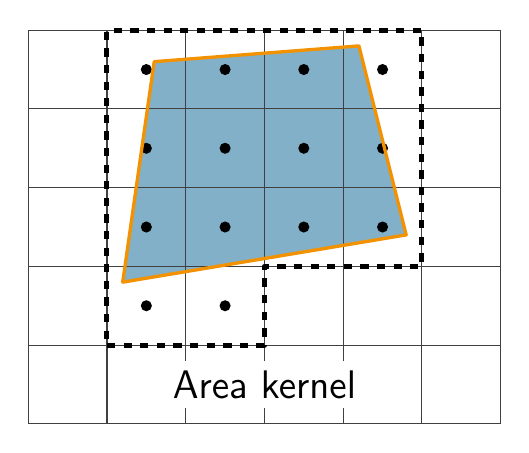
\begin{tikzpicture}[x=1cm,y=1cm]

    % -------------------------------------------------
    % White background
    % -------------------------------------------------
    \fill[white] (0,0) rectangle (6,5);

    % -------------------------------------------------
    % Quadrilateral interior
    %
    % The vertices are listed counter-clockwise:
    % (1.2,0.8), (4.8,1.4), (4.2,4.1), (1.6,3.6)
    % -------------------------------------------------
    \fill[xDarkBox]
        (1.2,1.8) --
        (4.8,2.4) --
        (4.2,4.8) --
        (1.6,4.6) -- cycle;

    % -------------------------------------------------
    % Background pixel grid
    %
    % This is deliberately drawn after the blue fill,
    % so that the grid lines remain visible inside the quad.
    % -------------------------------------------------
    \draw[
        step=1cm,
        darkgray,
        thin
    ] (0,0) grid (6,5);

    % -------------------------------------------------
    % Black dots in all pixels having non-zero overlap
    % with the quadrilateral.
    %
    % The dots are placed at the centers of those pixels.
    % -------------------------------------------------
    \foreach \x/\y in {
        1/1, 2/1,
        1/2, 2/2, 3/2, 4/2,
        1/3, 2/3, 3/3, 4/3,
        1/4, 2/4, 3/4, 4/4
    }{
        \fill[black] (\x+0.5,\y+0.5) circle (2pt);
    }

        % -------------------------------------------------
    % Dashed outer border of all marked pixels
    % -------------------------------------------------
    \draw[
        black,
        dashed,
        line width=1.8pt,
        line join=round
    ]
        (1,1) --
        (3,1) --
        (3,2) --
        (5,2) --
        (5,5) --
        (1,5) --
        cycle;
        
    % -------------------------------------------------
    % Orange quadrilateral boundary
    %
    % Drawn last so that the orange edges appear above
    % both the grid and the blue interior.
    % -------------------------------------------------
    \draw[
        xOrange,
        very thick,
        line join=round
    ]
        (1.2,1.8) --
        (4.8,2.4) --
        (4.2,4.8) --
        (1.6,4.6) -- cycle;

  \node[fill=white] (text) at (3,0.5) {\Large Area kernel};
\end{tikzpicture}

\end{document}
